
\subsection{CIVIS Back-end as a JS Runtime Environment}

The YouPower back-end is developed using the \textit{Node.js}\footnote{\url{https://nodejs.org/}} platform, a well-known JS based open source runtime environment for server-side applications. 
The platform is easily extensible and has a repository of libraries that support fast web development. 
% 
TU Delft prepared a virtual machine for CIVIS to host the WP3 back-end\footnote{\url{http://civis.tbm.tudelft.nl}}
using \textit{Nginx}\footnote{\url{https://nginx.org/en/}}, an http and reservse proxy server. 
% 
A \textit{Comodo}\footnote{\url{https://ssl.comodo.com/}} SSL certificate is installed on the server to provide secure communication (i.e. https). 

% 
The WP3 back-end interacts with the WP4 back-end, from which the former fetches relevant energy data that is particularly relevant for visualization of energy consumption/production and energy consumption signal. The availability of such data through the WP4 platform represents therefore a pre-condition for the ability of the app to correctly visualize such information.

\textit{MongoDB}\footnote{\url{https://mongodb.org/}} is used as the back-end database. It is document-oriented, and has flexible data schema and expressive query language. 
A list of the data models at the back-end can be found at {\footnotesize\url{https://github.com/CIVIS-project/YouPower/tree/master/backend/models}}. 
Figure~\ref{fig:datamodel} shows the data model schema.
%
\begin{figure}
\centering
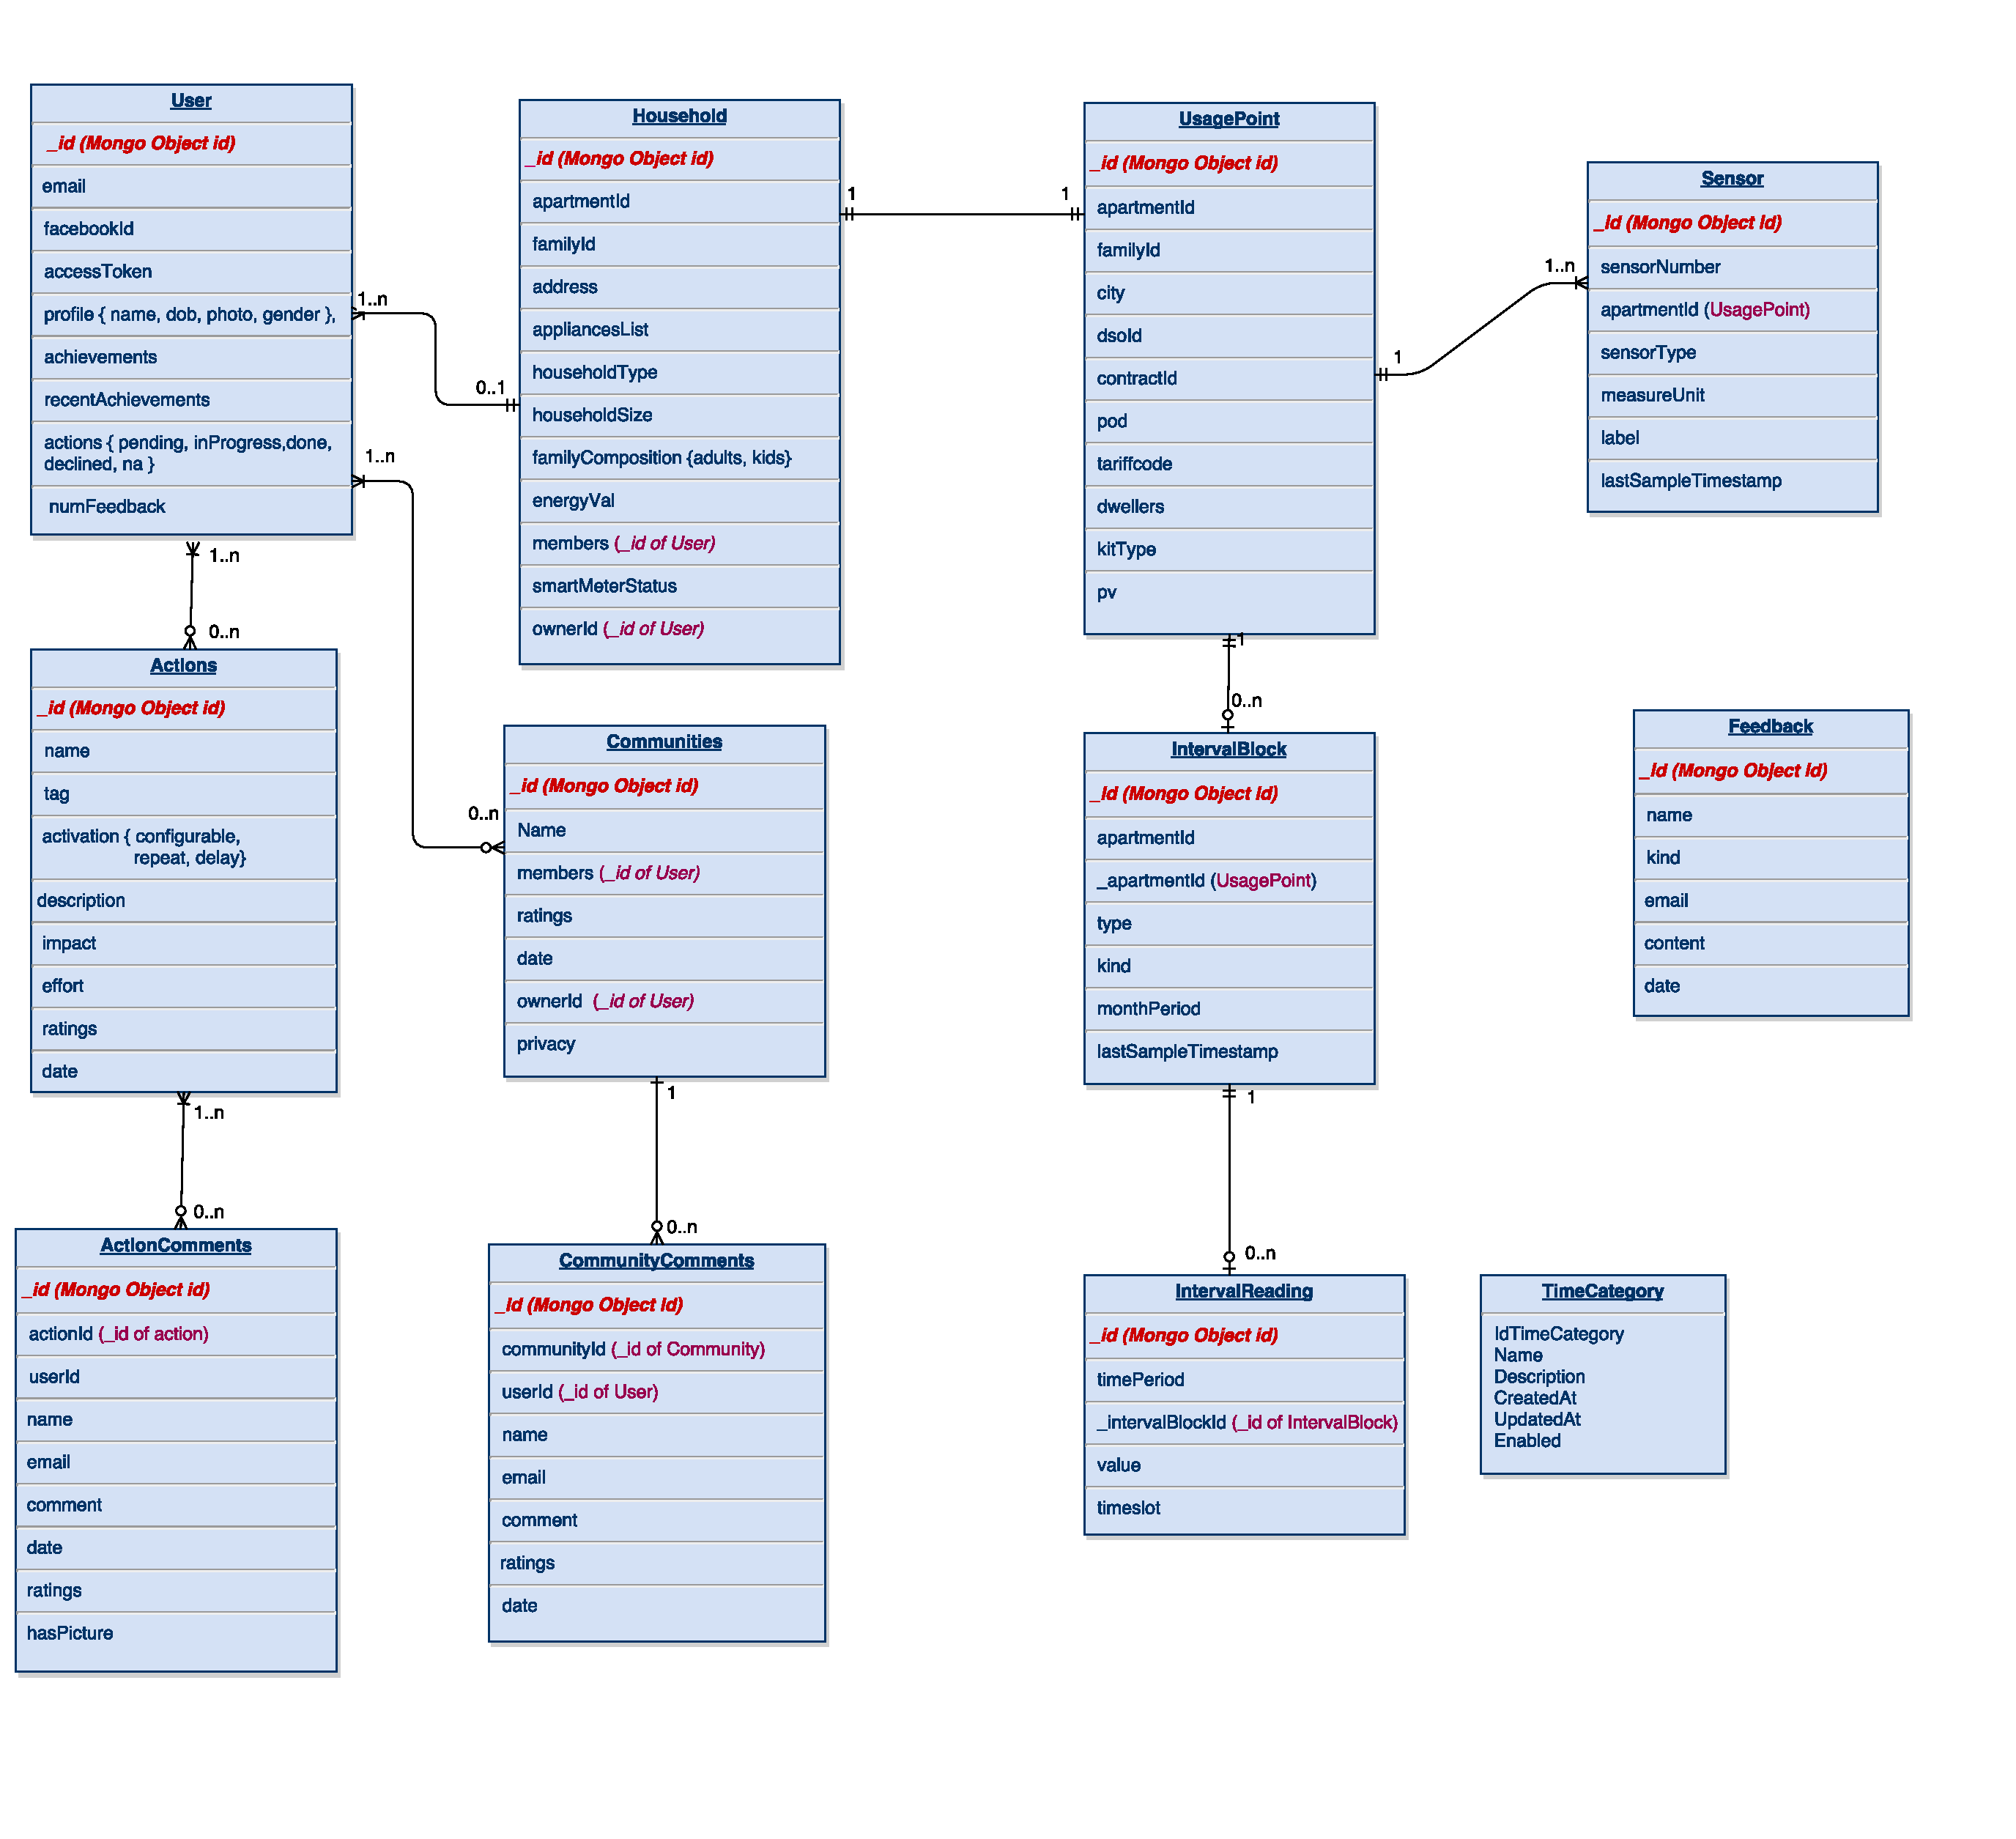
\includegraphics[height=\linewidth,angle=90]{img/datamodel_larger}
\caption{YouPower back-end data model schema}
\label{fig:datamodel}
\end{figure} 
% 

The noteworthy Node.js libraries used for the WP3 back-end development are as follows:

\begin{itemize}

\item Async.js\footnote{\url{https://github.com/caolan/async}}, which makes managing and combining asynchronous tasks easier. 

\item Express.js\footnote{\url{http://expressjs.com/}}, a Node.js application server framework we use as a basis for the REST API. 

\item Mocha\footnote{\url{https://mochajs.org/}}, a JavaScript unit test framework. 

\item Mongoose\footnote{\url{http://mongoosejs.com/}}, a MongoDB driver for Node.js. It provides a schema-based solution to model data. 

\item Passport.js\footnote{\url{http://passportjs.org/}}, for handling authentication of REST API requests for Node.js, both local (username password) and Facebook. 

\item Underscore.js\footnote{\url{http://underscorejs.org/}}, a JS library that provides over 100 utility functions. 
%\item Ionic Push\footnote{\url{https://apps.ionic.io/landing/push}}, for sending dynamic push notifications. 

\item Nodemailer\footnote{\url{https://nodemailer.com/}}, sending emails with Node.js.

\item Email-templates\footnote{\url{https://www.npmjs.com/package/email-templates}}, a Node.js module for rendering beautiful emails.

\item Fb\footnote{\url{https://www.npmjs.com/package/fb}}, a Node.js library for Facebook.

\item Moment.js\footnote{\url{http://momentjs.com/}}, a JS library to parse, validate, manipulate and display dates. 

\item APIDOC script\footnote{\url{http://apidocjs.com/}}, for inline documentation for the REST API. 
\end{itemize}

The YouPower back-end REST API documentation can be found at {\footnotesize\url{http://civis.tbm.tudelft.nl/apidoc/}}. 
% 


\subsection{Feature enhancements (Frontend and Backend)}
We added substantial feature for visualizing the energy consumption and production of households in Trentino test sites, CEIS and CEDIS. We have developed a number of endpoints that interacts with Reply and  TOU signals from CreatNet. In the following sub sections, we described the endpoints we have developed and API path while details on the new endpoints description and parameter list could be found in the API documentation of YouPower.

\subsubsection{Accessibility}
The energy tab is only visible for users from trentino test site. Users should select their  corresponding municipality area (i.e. CEIS or CEDIS) and provide a contract Id in the settings page. This contract Id will then be mapped to Apartment ID (also called UsagePoint). Apartment Id is unique for each household and data associated with consumption and production recorded from the sensor are referenced through  this Ids.

\subsubsection{TOU (Time of Use) signals}
YouPower provides the current energy level(red smileys representing  low energy  tariffs and green smiley for high energy tariff levels) and a prediction of energy tariff levels for the following 30 hours. TOU signals are provided with a non-secured protocol(http) which raises mixed content issue since YouPower requires a secure connection. For this, we have developed two backend APIs.

\begin{table}[h!]
\caption{TOU endpoints}\label{tab:app_nav}
\begin{center} \footnotesize 
\begin{tabular}{ l p{6cm}}
\hline
\textbf{Endpoint}  &
\textbf{Description}  \\ \hline

/api/energymeteo/tou  & 
Provides energy level tariffs for previous 30 hours
\\ 
/api/energymeteo/tou/current & Provides the current energy tariff \\ 
 \hline
\end{tabular}
\end{center} 
\end{table}

\subsubsection{Electric consumption and production updates}
The app update users by showing the amount of consumption and production in a given time(energy) and power levels of the last six to eight minutes recorded in either today or the last time a sensor provides this informations. Sometimes, when there is a sudden changes in power, raspberry may need  to restart or  lack of connectivity to internet may happen. In this cases, sensors may stop sending signals to the Reply server. The app shows the most recent updates that shows the last time an electric consumption and production recorded from sensors.

\subsubsection{Appliances consumption updates}
The app includes information on consumption per each appliance. List of all available appliances for a household like ``Lavatrice'' and ``Freezer'' are listed in the appliances tab of the app, with corresponding timing where last consumption is recorded.
\begin{table}[h!]
\caption{Endpoints for getting last consumption records}\label{tab:app_nav}
\begin{center} \footnotesize 
\begin{tabular}{ l p{6cm}}
\hline
\textbf{Endpoint}  &
\textbf{Description}  \\ \hline


/api/consumption/last
  & 
Provides energy level tariffs for previous 30 hours \\ 
/api/production/last & Provides the last production amount recorded for a household with a PV \\ 
/api/consumption/appliance & Gives list of all available appliances for a household and the last time stamp a consumption data is recorded \\ 
 \hline
\end{tabular}
\end{center} 
\end{table}
\subsubsection{Energy data(Consumption and production)
}
Daily consumption provided by an appliance is accessible from YouPower by setting a range of dates (users can avoid sending unnecessary request of a consumption which may not be available by checking the recent updates) a user is interested at. A series of consumption history for all the appliances of a household can also be obtained by requesting the endpoint with a contract Id.
\begin{table}[h!]
\caption{Endpoints for getting energy consumption}\label{tab:app_nav}
\begin{center} \footnotesize 
\begin{tabular}{ l p{6cm}}
\hline
\textbf{Endpoint}  &
\textbf{Description}  \\ \hline

/api/consumption/appliance/:applID
  & 
Provides the consumption history of an appliance taking household Id, startdate and enddate as parameters \\ 
/api/consumption & Provides a series of consumption history for all appliances of a household in F1, F2 and F3 levels \\ 
 \hline
\end{tabular}
\end{center} 
\end{table}

\subsubsection{Consumption comparison in energy tariff levels}
This part of the app shows comparison containing consumption record of a household based on red and green levels. The red levels shows the amount of consumption a household used when the energy level is low, and the green for high energy levels.

\subsubsection{Community consumption comparison}
This section contains two main comparison graphs. The first contains consumption comparison of the two municipalities, CEIS and CEDIS, for the 24 hours period of the required date in intervals of 1 hour. The second part of the graph shows comparison of a household consumption with the total consumption of a municipality and the average consumption of the households in the same municipality. We implemented an endpoint for accessing the daily consumption of all households from reply server and it will be dumped to Delft server for accessing requested resource fast.

\subsubsection{Technical issues}
We have used the same set of technologies stated in the Backend section of this document. We have listed the issues we have faced during feature improvement.
\begin{table}[h!]
\caption{Technical issues}\label{tab:app_nav}
\begin{center} \footnotesize 
\begin{tabular}{ l p{6cm}}
\hline
\textbf{Issue}  &
\textbf{Status}  \\ \hline

DatePicker incompatibility with firefox
  & 
Not fixed -- planned for next update\\ 
CORS issue when accessing CN endpoints & Fixed: CN server allow civisproject domain \\ 
 \hline
\end{tabular}
\end{center} 
\end{table}


\subsection{Resources}